%##################################################################################################

The tasks under the \texttt{craft} category in our benchmark have been designed to shed light on an AI agent's prowess in item utilization, the intricacies of Minecraft crafting mechanics, and the nuances of various game mechanic interactions. These tasks provide a detailed examination of an agent's capability to convert materials into functional items and harness the game's various crafting and enhancement mechanics. 

\begin{figure*}[h]
%\framebox[4.0in]{$\;$}
\begin{center}
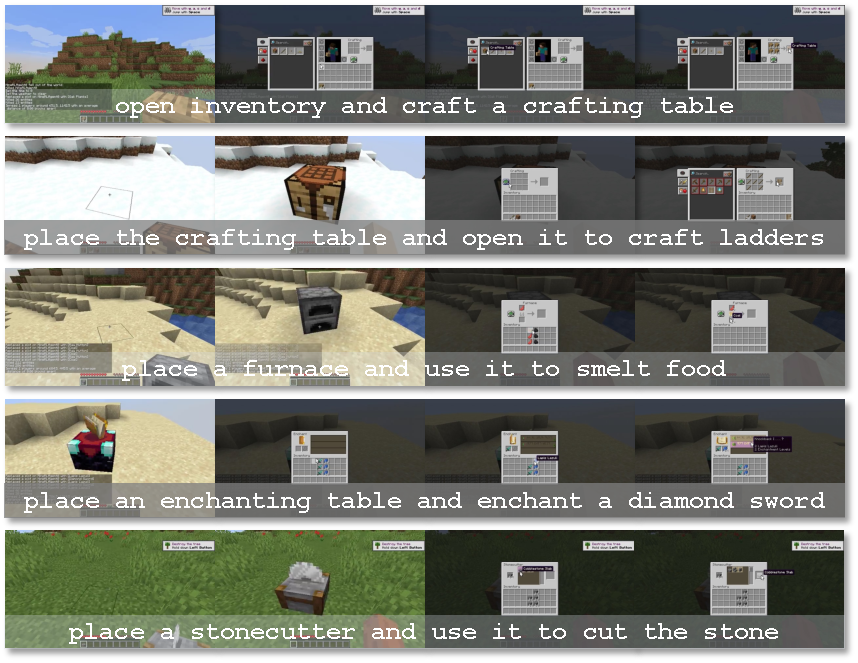
\includegraphics[scale = 0.9]{figures/benchmark_craft.pdf}
\end{center}
\caption{Examples of tasks in \texttt{craft} category. }
\end{figure*}


\definecolor{codeblue}{rgb}{0.25,0.5,0.5}
\definecolor{codekw}{rgb}{0.85, 0.18, 0.50}
\definecolor{keywordgreen}{rgb}{0,0.6,0}
\lstset{
  backgroundcolor=\color{gray!10},
  basicstyle=\fontsize{8pt}{9pt}\ttfamily\selectfont,
  columns=fullflexible,
  breaklines=true,
  captionpos=b,
  commentstyle=\fontsize{7.5pt}{7.5pt}\color{codeblue},
  keywords = {Task, Description, Time, Evaluation, Precondition, SkillAssessed}, 
  keywordstyle = {\textbf},
  caption={The environment configuration and evaluation metric for \texttt{craft} series tasks. },
  label={lst:minecraft_deps_prompt}
}
\begin{lstlisting} % [language=python]  

Task: craft the crafting_table
Description: Open inventory and craft a crafting table. 
Precondition: Spawn the player in the plains biome with a stack of oak_planks in the inventory. 
SkillAssessed: Inventory management and basic crafting.
Evaluation: Open the inventory. < Click on the recipe button. < Click on the crafting_table. < Drag the crafting_table into the inventory. 

Task: craft ladders 
Description: Place the crafting table and open it to craft ladders. 
Precondition: Spawn the player in the plains biome with a crafting_table in its main hand and a stack of oak_planks in the inventory. 
SkillAssessed: Advanced crafting using crafting stations and recipe navigation.
Evaluation: Place the crafting_table on the surface. < Open the crafting_tabe. < Click on the recipe book. < Click on the ladder. < Drag the ladder into the inventory. 

Task: enchant sword
Description: Place an enchanting table and use it to enchant a diamond sword. 
Precondition: Spawn the player in the plains biome with an enchanting table in its main hand, 3 diamond swords, and 3 stacks of lapis_lazuli in the inventory. 
SkillAssessed: Tool enhancement using enchantment stations and decision-making in choosing enchantments.
Evaluation: Place the enchanting_table on the surface. < Open the enchanting_table. < Place the lapis_lazuli or diamond sword. < Place the lapis_lazuli and diamond sword. < Choose any enchantment. 

Task: smelt food
Description: Place a furnace and use it to smelt food. 
Precondition: Spawn the player in the plains biome with a furnace table in its main hand, 3 stacks of mutton, and 3 stacks of coal in the inventory. 
SkillAssessed: Food processing using a smelting furnace, raw material to product conversion, and patience in awaiting outcomes. 
Evaluation: Place the furnace on the surface. < Open the furnace. < Place raw meat or coal. < Place both raw meat and coal. < Wait for the raw meat to be cooked. < Take out cooked meat. 

Task: cut stone
Description: Place a stonecutter and use it to cut stones. 
Precondition: Spawn the player in the plains biome with a stonecutter in its main hand, 6 stacks of stones in the inventory. 
SkillAssessed: Tool enhancement using enchantment stations and decision-making in choosing enchantments.
Evaluation: Place the stonecutter on the surface. < Open the stonecutter. < Place the stones. < Select a target type of stone. < Drag stones to the inventory. 

\end{lstlisting}

